\section{传统主——谓命题}

\begin{quotation}
本节探讨传统逻辑中的四种主谓命题形式及其符号化表示。通过分析全称肯定、全称否定、特称肯定和特称否定命题的结构,我们将学习如何用量词和命题函项准确表达它们,并理解这些命题形式之间的逻辑关系,从而增强对自然语言与符号逻辑之间转换的理解。
\end{quotation}

\subsection{四种基本命题形式}

运用存在和全称量词,以及根据对图 10-1 中对当方阵的理解,我们现在开始分析(并且在推理中准确地使用)以下四种为传统逻辑研究所注重的普遍命题。这四种命题的标准例子如下:

\begin{center}
\begin{tabular}{ll}
所有人是有死的。 & [全称肯定:A] \\
所有人都不是有死的。 & [全称否定:E] \\
有些人是有死的。 & [特称肯定:I] \\
有些人不是有死的。 & [特称否定:O] \\
\end{tabular}
\end{center}

每种命题通常由其字母来指称:两种肯定命题用 A 和 I(来自拉丁文\\
affirmo,我肯定);两种否定命题用 E 和 O (来自拉丁文 nego,我否认)。\cite{peirce1883}

\subsection{A型命题的符号化}

用量词符号化这些命题,使得我们进一步扩大了命题函项概念。首先来看 \textbf{A命题}"所有人是有死的",我们从下述命题开始逐次解释:

给定不管任何事物,如果它是人,它是有死的。

其中关系代词"它"的两次出现显然是回指它们共同的先行词"事物"。与上节的前部分一样,因为它们有同样的(不确定的)指称,从而都能用字母"$x$"替换。于是该命题可改写成:

给定任何 $x$ ,如果 $x$ 是人,那么 $x$ 是有死的。

现在,用先前引入的"如果一那么"的符号,可以把前一个命题改写成:

给定任何 $x, x$ 是人 $\supset x$ 是有死的。

最后,用我们已掌握的命题函项符号和量词,原来的 A 命题可表示为:

$$
(x)(H x \supset M x)
$$

在我们的符号翻译中, A 命题是以一种新的命题函项的全称量化形式出现的。表述式 $H x \supset M x$ 是一个命题函项,它既没有单称肯定命题又没有单称否定命题作为其代人例,而是以条件陈述作为代人例,这些条件陈述的前件和后件是具有同样主项的单称命题。命题函项 $H x \supset M x$ 的代人例有条件陈述 $H a \supset M a 、 H b \supset M b 、 H c \supset M c 、 H d \supset$ $M d$ 等等。

另一些命题函项则以有同样主项的单称命题的合取为代入例。例如, $H a \cdot M a 、 H b \cdot M b 、 H c \cdot M c 、 H d \cdot M d$ 等等都是命题函项 $H x \cdot M x$ 的代人例。还有一些形如 $W x \vee B x$ 的命题函项,它们的代入例是诸如 $W a \vee$ $B a$ 和 $W b \vee B b$ 这样的析取式。实际上,任何以具有相同主项的单称命题为分支陈述的真值函项复合命题,都可以看做由某些或所有真值函项联结词(圆点号、楔劈号、马蹄号、三杠等值号和波浪号)加之简单谓词\\
( $A x 、 B x 、 C x 、 D x \cdots \cdots$ )所构成的命题函项的代人例。在把 A 命题翻译成( x )( $H \mathrm{x} \supset M x$ )时,圆括号充当标点符号,用以表明全称量词( $x$ ) "作用于"整个(复合)命题函项 $H x \supset M x$ ,或命题函项 $H x \supset M x$"作为其辖域"。

在继续讨论直言命题的其他传统形式之前,应该注意符号公式( $x$ ) ( $H x \supset M x$ )不仅是对标准形式的命题"所有 $H$'s 都是 $M$'s"的翻译,而且是对任何一个有同样含义的自然语言句子的翻译。\cite{brown1954} 在自然语言中,述说这同一件事有许多不同的方式。它们的部分清单如下:"$H$ 是 $M$","一个 $H$ 就是一个 $M$","每个 $H$ 是 $M$","每一个 $H$ 是 $M$","任何 $H$ 是 $M$", "没有 $H$ 不是 $M$","是 $H$ 的每个事物都是 $M$","是 $H$ 的任何事物都是 $M "$ ,"如果任何事物是 $H$ ,那么它是 $M$","如果某事物是 $H$ ,那么它是 $M$","是 $H$ 的无论什么东西都是 $M$","$H$'$s$ 全都是 $M$'$s$","只有 $M$'$s$ 是 $H^{\prime} s "$ ,"除了 $M^{\prime} s$ 以外,没什么是 $H^{\prime} s "$ ,"没什么是 $H$ ,除非它是 $M^{\prime}$",以及"没有什么是 $H$ 但不是 $M$"。再者,同一含义的命题可以用抽象名词表达:"人蕴涵(或涵衍)有死"可以正确地符号化为一个 A 命题。符号逻辑语言对相当数量的自然语言句子的共同含义有一个单一的表达式,这一点被认为是符号逻辑在认知或信息方面比自然语言优越之处,一一尽管从修辞力或诗意表现的观点看,我们承认这是一种劣势。 

\subsection{其他类型命题的符号化}

\textbf{E命题}"所有人都不是有死的"可以被依次释为:

\begin{quote}
给定不管任何个体事物,如果它是人,那么它不是有死的。\\
给定任何 $x$ ,如果 $x$ 是人,那么 $x$ 不是有死的。\\
给定任何 $x, x$ 是人 $\supset x$ 不是有死的。
\end{quote}

最后可以释为:

$$
(x)(H x \supset \sim M x)
$$

这种符号翻译不仅表示了自然语言中传统的 E 形式,同样也表示了一些说同一件事的不同方式,如"没有是 $M$ 的 $H$","没有什么既是 $H$ 又是 $M$",以及"$H$ 从不是 $M$"。

同样,\textbf{I命题}"有些人是有死的"可以依次释为:

至少有一个是人且有死的事物。\\
至少有这样一个 $x, x$ 是人并且 $x$ 是有死的。\\
至少有这样一个 $x, x$ 是人• $x$ 是有死的。

进而可以释为:

$$
[(\exists x)(H x \cdot M x)]
$$

最后,\textbf{O命题}"有些人不是有死的"可以依次释为:

至少存在一个是人但不是有死的事物。\\
至少存在这样一个 $x, x$ 是人并且 $x$ 不是有死的。\\
至少存在这样一个 $x, x$ 是人• $\sim x$ 是有死的。

它可以完全符号化为:

$$
[(\exists x)(H x \cdot \sim M x)]
$$

\subsection{命题形式间的逻辑关系}

若用希腊字母 phi( $\phi$ )和 psi( $\Psi$ )表示任何一个谓词,传统逻辑的四个主—谓型普遍命题可以在图 10—2 所示的方阵中得到表达。\\
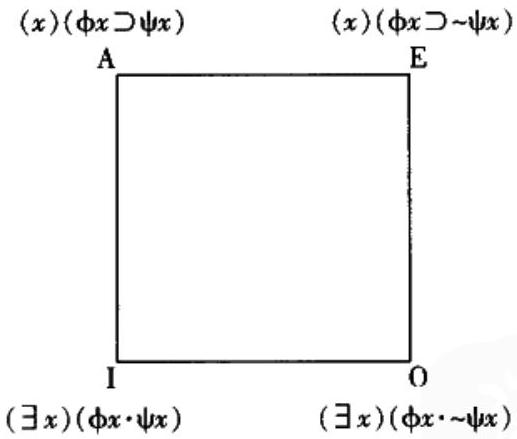
\includegraphics[width=\textwidth]{images/2025_05_15_6a28331d5e7c993ad07ag-466.jpg}

图10-2\\
显然, A 命题和 O 命题是\textbf{矛盾关系},一个是另一个的否定; E 命题和 I 命题也是矛盾关系。

有人可能会认为,一个 I 命题可以从与之相对的 A 命题推出,一个 O命题可以从与之相对的 E 命题推出,但情况并非如此。一个 A 命题为真时,与之对应的 I 命题却可能是假的。如果 $\phi_{x}$ 是一个没有真代人例的命

题函项,那么,不管命题函项 $\Psi x$ 有何种代人例,(复合)命题函项 $\phi_{x} \supset$ $\Psi x$ 的全称量化式都是真的。例如,考虑命题函项"$x$ 是一个人首马身的怪物",我们把它简写为 $C x$ 。因为不存在人首马身的怪物,$C x$ 的每个代入例都是假的,即 $C a 、 C b 、 C c \cdots \cdots$ 都为假。因此,复合命题函项 $C x \supset B x$的每个代人例都是一个前件为假的条件陈述。这样,其代人例 $\mathrm{Ca} \supset \mathrm{Ba}$ 、 $C b \supset B b 、 C c \supset B c$ 都是真的,因为任何一个断言实质蕴涵的条件陈述,如果其前件为假,那么它必定为真。由于其所有代人例都是真的,所以,命题函项 $C x \supset B x$ 的全称量化式为真,即 A 命题 $(x)(C x \supset B x)$ 为真。但与之相对的 I 命题 $(\exists x)(C x \cdot B x)$ 却是假的,因为命题函项 $C x \cdot B x$没有真代人例。 $C x \cdot B x$ 没有真代人例可以从 $C x$ 没有真代人例推出。 $C x \cdot B x$ 的各个代人例,如 $C a \cdot B a 、 C b \cdot B b 、 C c \cdot B c \cdots \cdots$ 都是第一个合取支为假的合取式,因为 $C a 、 C b 、 C c \cdots \cdots$ 都为假。由于其所有代人例都为假,所以命题函项 $C x \cdot B x$ 的存在量化式为假,即 I 命题( $\exists x$ )( $C x \cdot B x$ )为假。因此,有可能一个 A 命题是真的,而与之对应的 I 命题却是假的。

这种分析还可表明,为什么有可能一个 E 命题是真的,而与之对应的 $O$ 命题却是假的。如果我们以命题函项 $\sim B x$ 替换前面讨论中的命题函项 $B x$ ,那么,$(x)(C x \supset \sim B x)$ 可以是真的,而 $(\exists x)(C x \cdot \sim B x)$ 却是假的。当然,这也是因为并没有人首马身的怪物。

\subsection{命题类型间的关键区别}

问题的关键在于:A 命题和 E 命题并不断言或假定任何事物存在,它们仅断言情况是这样的:如果有某事,则有另外一件事。但 I 命题和 O 命题却假定某物存在,它们断言情形是这样的:有这件事并且有另一件事。 1 命题和 $O$ 命题中的\textbf{存在量词}是区别的关键所在。从一个并不断言或假定任何事物存在的命题推出某物的存在,这显然是错误的。

如果我们假定至少有一个个体存在,那么( $x$ )( $C x \supset B x$ )确实蕴涵 ( $\exists x) ~(C x \supset B x)$ 。但后者不是一个 I 命题。 I 命题"有些人首马身的怪物是漂亮的"应符号化为 $(\exists x)(C x \cdot B x)$ ,它说的是,至少存在一个漂亮的人首马身的怪物。但在自然语言中,被符号化为( $\exists x$ )( $C x \supset B x$ )的东西,可以被理解为"至少存在一个如此这般的事物,如果它是人首马身的怪物,那么它是漂亮的"。它并没说存在一个人首马身的怪物,而只是说存在一个个体,它或者不是人首马身的怪物,或者是漂亮的。而这个命题只在两种情况下是假的:第一,如果根本不存在个体;第二,如果所有个体都是人首马身的怪物,并且它们当中没有一个是漂亮的。通过作这样

一个明确的(并且显然是真的)假定,即假定宇宙中至少存在一个个体,我们可以排除第一种情形。第二种情形是如此极端地不合理,以致与 I 形命题( $\exists x$ )( $\phi_{x} \cdot \Psi x$ )的重要性相反,任何形如( $\exists x$ )( $\phi_{x} \supset \Psi x$ )的命题都必定是非常平庸的。显而易见,尽管在自然语言中 A 命题"所有人是有死的"和 I 命题"有些人是有死的"的区别,仅在于初始词"所有"和"有些"的不同,但它们意义上的区别并不限于全称量化和存在量化,而是比这深刻得多。经量化而产生 A 命题和 I 命题的命题函项不仅在量化上有区别,而且它们还是不同的命题函项,一个含有"$\supset$",另一个含有"•"。换言之,A 命题和 I 命题并不像它们在自然语言中看起来那么相似。它们之间的区别可通过使用命题函项符号和量词符号得以彰显。

\subsection{命题变形技巧}

就逻辑操作来说,处理那些否定号的出现——如果有否定号出现的话——只作用于简单谓述的公式最为方便。因此,我们将在必要时通过替换来得到这种公式。要做到这一点很简单。从第9章所确立的推论规则可知,我们可以用另一个与之逻辑等价的表述式来替换一个表述式。而我们有四个这样的逻辑等价式(10.2节),它们当中否定号在量词之前的命题,都与另一个否定号直接作用于简单谓述的命题等价。用我们熟悉已久的推论规则,可以移动否定号,使它们最终不再作用于复合表达式,而只作用于简单谓述。譬如说,公式:

$$
\sim(\exists x)(F x \cdot \sim G x)
$$

可以依次改写。首先,如果我们用 10.2 节所给的第三个逻辑等价式,它可以变形为:

$$
(x) \sim(F x \cdot \sim G x)
$$

然后,可运用德摩根律使之变成:

$$
(x)(\sim F x \vee \sim \sim G x)
$$

再用双重否定律可得公式:

$$
(x)(\sim F x \vee G x)
$$

最后,若援引实质蕴涵定义,原公式也可以改写成下述 A 命题:

$$
(x)(F x \supset G x)
$$

在转到关于非复合陈述推论的话题之前,读者应该进行一些把非复合陈述从自然语言翻译成逻辑符号的训练。自然语言有如此之多不规则的和惯用的构造,以致不可能有把自然语言语句翻译成逻辑符号的简单规则。在任何情形下都要先理解语句的含义,然后用命题函项和量词术语予以重述。

\begin{center}
\fbox{\parbox{0.95\textwidth}{
\textbf{本节要点}
\begin{itemize}
\item \textbf{传统四种命题形式}:
  \begin{itemize}
  \item A型(全称肯定):所有S是P,符号化为(x)(Sx⊃Px)
  \item E型(全称否定):所有S都不是P,符号化为(x)(Sx⊃~Px)
  \item I型(特称肯定):有些S是P,符号化为(∃x)(Sx·Px)
  \item O型(特称否定):有些S不是P,符号化为(∃x)(Sx·~Px)
  \end{itemize}
\item \textbf{符号化的结构差异}:
  \begin{itemize}
  \item A型和E型命题使用条件结构(⊃)和全称量词
  \item I型和O型命题使用合取结构(·)和存在量词
  \item 这种结构差异揭示了自然语言中隐含的逻辑区别
  \end{itemize}
\item \textbf{命题间的逻辑关系}:
  \begin{itemize}
  \item A与O、E与I构成矛盾关系(一真一假)
  \item A命题不必然蕴涵I命题(当主词类为空时)
  \item E命题不必然蕴涵O命题(当主词类为空时)
  \end{itemize}
\item \textbf{存在假定的区别}:
  \begin{itemize}
  \item A型和E型命题不假定主词类存在
  \item I型和O型命题假定主词类有实例存在
  \item 这一区别解释了为何A型命题不必然蕴涵I型命题
  \end{itemize}
\end{itemize}
}}
\end{center}
